\begin{figure*}[t]
\centering
\begin{minipage}[t]{0.52\textwidth}
\vspace{0pt}
{\small\bfseries (a) Training graph}\par\smallskip
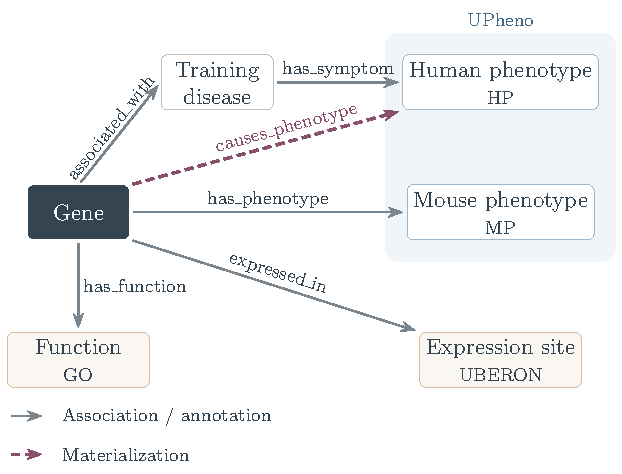
\includegraphics[width=\linewidth]{fig/overview_graph_clean.pdf}
\end{minipage}\hfill
\begin{minipage}[t]{0.44\textwidth}
\vspace{0pt}
{\small\bfseries (b) Per-gene calibration}\par\smallskip
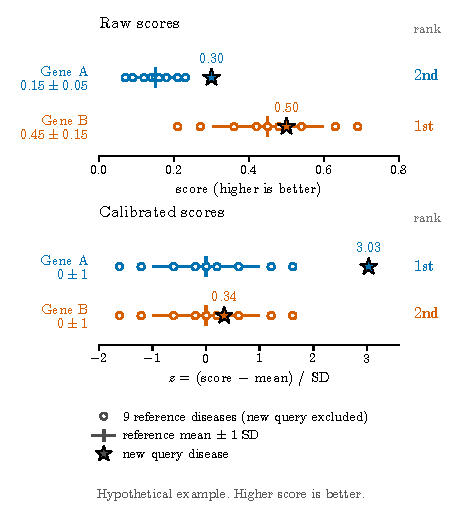
\includegraphics[width=\linewidth]{fig/fig_calibration.pdf}
\end{minipage}
\caption{Overview of \method{}.
(a) Solid arrows show training associations and annotations.
The dashed purple edge materializes the gene--disease--phenotype path
as a \texttt{causes\_phenotype} triple. The UPheno region groups
MP and HP phenotype classes; ontology hierarchy edges are omitted.
(b) Per-gene calibration. A candidate gene's score for the new disease is
standardized by subtracting that gene's mean and dividing by its standard
deviation over reference scores; the example illustrates the resulting rank
reversal. Evaluation uses one reference vector per distinct disease and
leaves out the query disease. A fixed training-disease panel is evaluated
separately.}
\label{fig:overview}
\end{figure*}
